\documentclass[12pt, legalpaper]{exam}
\usepackage[utf8]{inputenc}
\usepackage[english]{babel}
\usepackage[margin=.8in]{geometry}
\usepackage{amsmath,amssymb}
\usepackage{multicol}
\usepackage{graphicx}
\usepackage{tikz}
\usepackage{lastpage}
\usepackage{tabularx}
\usepackage{hyperref}
\usepackage{tcolorbox}
\usepackage{hyperref}
\hypersetup{
    colorlinks=true,
    linkcolor=blue,
    filecolor=magenta,      
    urlcolor=cyan,
    pdftitle={Overleaf Example},
    pdfpagemode=FullScreen,
    }
\newcommand{\course}{Introduction to Optimization}
\newcommand{\term}{Fall 2023}
\newcommand{\examnum}{Report of Programming Task 1}


\begin{document}
\noindent \examnum \, of the  course ''\course'' - \term


\noindent
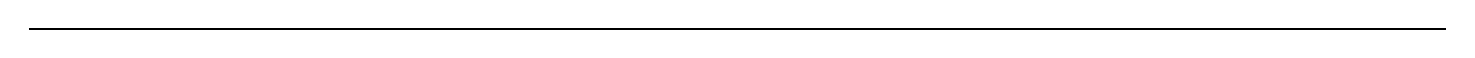
\begin{tikzpicture}
\draw[thick] (0,0) -- (18,0);
\end{tikzpicture}




\vspace{12pt}
\begin{center}
    \textbf{Report 1}
\end{center}
% \noindent \textbf{Requirements}

\vspace{12pt}

\noindent  \textbf{Team information.}

\begin{itemize}
    \item Team leader: Roman Pogrebnyak
    \item Team member 1: Maksim Kamenetskii
    \item Team member 2: Möe Jaafar
    \item Team member 3: Feliks Cherdzhiev
    \item Team member 4: Bahdan Shakh
\end{itemize}
\vspace{12pt}
\noindent     \textbf{Link to the product.}
\begin{itemize}
    \item The product is available: \href{https://github.com/OptimizationAssignmentsIU3Sem/Simplex_assignment1/tree/main}{Link to GitHub}
\end{itemize}

\vspace{12pt}

\noindent  \textbf{Programming language.}
\begin{itemize}
    \item Programming language: Python
\end{itemize}

\vspace{12pt}

\noindent  \textbf{Linear programming problem.}
\begin{itemize}
\item Maximization
\vspace{10pt}
    \item Objective function:
    \vspace{10pt}
    \item Constraint functions:
    \vspace{5cm}
\end{itemize}



\noindent     \textbf{Input}

\vspace{12pt}
The input contains:
\begin{itemize}
    \item A vector of coefficients of objective function - $C$.
    \item A matrix of coefficients of constraint function - $A$.
    \item A vector of right-hand side numbers - $b$.
    \item The approximation accuracy $\epsilon$.
\end{itemize}

\vspace{12pt}
\noindent     \textbf{Output/Results}

The output contains:
\begin{itemize}
    \item The string "The method is not applicable!"
    
or

    \item A vector of decision variables - $X^*$.
    \item Maximum (minimum) value of the objective function.
\end{itemize}

\noindent
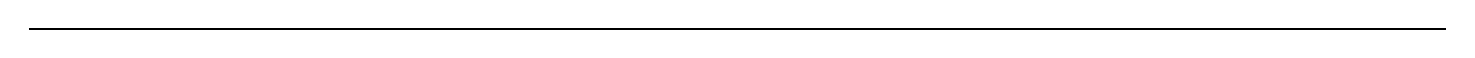
\begin{tikzpicture}
\draw[thick] (0,0) -- (18,0);
\end{tikzpicture}




\vspace{24pt}
\noindent     \textbf{Code}

Copy-paste your code here.


\end{document}
